\documentclass[11pt,a4paper]{article}
\usepackage[utf8]{inputenc}
\usepackage[T1]{fontenc}
\usepackage{geometry}
\usepackage{graphicx}
\usepackage{booktabs}
\usepackage{array}
\usepackage{longtable}
\usepackage{float}
\usepackage{amsmath}
\usepackage{amssymb}
\usepackage{hyperref}
\usepackage{xcolor}
\usepackage{listings}
\usepackage{enumitem}
\usepackage{pgfplots}

\geometry{margin=1in}
\pgfplotsset{compat=1.18}

\definecolor{codebg}{RGB}{248,248,248}
\definecolor{codegray}{RGB}{90,90,90}
\definecolor{codeblue}{RGB}{0,92,197}
\definecolor{codegreen}{RGB}{0,120,70}

\lstdefinestyle{thesisstyle}{
  backgroundcolor=\color{codebg},
  basicstyle=\ttfamily\small,
  commentstyle=\color{codegray},
  keywordstyle=\color{codeblue}\bfseries,
  stringstyle=\color{codegreen},
  breaklines=true,
  frame=single,
  rulecolor=\color{black!15},
  tabsize=2,
  showstringspaces=false,
  columns=fullflexible
}

\lstset{style=thesisstyle}

\hypersetup{
  colorlinks=true,
  linkcolor=blue,
  urlcolor=blue,
  citecolor=blue,
  pdftitle={Phase 3 Progress Report},
  pdfauthor={Deep Shukla}
}

\title{Week 5--6 Progress Report\\Prototype Implementation and System Demonstration}
\author{Deep Shukla}
\date{April 19, 2026}

\begin{document}

\maketitle

\section{Introduction}

This Phase 3 document reports the implemented prototype of the Swiss Open Government Data (OGD) fuzzy retrieval system. The prototype operationalizes the system design developed in the earlier phases and demonstrates the complete retrieval pipeline from query processing to fuzzy ranking, explanation generation, and baseline comparison.

The implementation is aligned with the thesis scope stated in the repository documentation: handling vague search intent, incorporating metadata quality into ranking, supporting multilingual queries, and providing interpretable results. The current codebase also includes a Streamlit-based prototype interface, CKAN API integration, a Mamdani fuzzy inference engine, a query parser, ranking modules, and evaluation artifacts.

\section{Phase 3 Objectives}

The main objectives for Phase 3 are:
\begin{enumerate}[leftmargin=1.5em]
  \item Implement the end-to-end prototype in Python.
  \item Connect the prototype to the Swiss OGD CKAN API.
  \item Process user queries and extract intent-related signals.
  \item Compute ranking features such as similarity, recency, completeness, and resource availability.
  \item Apply fuzzy inference to produce an interpretable relevance score.
  \item Generate explanations for ranking decisions.
  \item Validate the implementation with integration tests and prototype outputs.
\end{enumerate}

\section{Implemented Prototype Structure}

The current implementation is organized into the following modules:

\begin{table}[H]
\centering
\begin{tabular}{p{0.28\textwidth} p{0.64\textwidth}}
\toprule
\textbf{Module} & \textbf{Role} \\
\midrule
\texttt{\detokenize{code/main.py}} & Command-line entry point for prototype, demo, and data collection. \\
\texttt{\detokenize{code/prototype/app.py}} & Thin wrapper that launches the Streamlit prototype. \\
\texttt{\detokenize{code/prototype/swiss_ogd_portal.py}} & Main interactive prototype UI and ranking workflow. \\
\texttt{\detokenize{code/data_collection/ckan_api_client.py}} & CKAN API client for opendata.swiss metadata retrieval. \\
\texttt{\detokenize{code/query_processing/query_parser.py}} & Query parsing, language detection, and intent extraction. \\
\texttt{\detokenize{code/query_processing/llm_normalizer.py}} & Optional query normalization layer. \\
\texttt{\detokenize{code/fuzzy_system/inference_engine.py}} & Mamdani fuzzy inference engine. \\
\texttt{\detokenize{code/fuzzy_system/fuzzy_rules.py}} & Rule base used by fuzzy inference. \\
\texttt{\detokenize{code/ranking/fuzzy_ranker.py}} & Ranking orchestration and metadata scoring. \\
\texttt{\detokenize{code/ranking/baseline_keyword.py}} & Keyword retrieval baseline. \\
\texttt{\detokenize{code/ranking/ai_semantic_baseline.py}} & Semantic baseline for comparison. \\
\texttt{\detokenize{code/ranking/explanation_generator.py}} & Human-readable ranking explanations. \\
\texttt{\detokenize{evaluation/evaluation_framework.py}} & Evaluation workflow and metrics. \\
\texttt{\detokenize{evaluation/experiment_runner.py}} & Experiment execution and result generation. \\
\bottomrule
\end{tabular}
\caption{Implemented prototype modules}
\end{table}

The wrapper entrypoint in \texttt{\detokenize{code/prototype/app.py}} launches \texttt{\detokenize{code/prototype/swiss_ogd_portal.py}}, which contains the interactive research prototype.

\section{Prototype Workflow}

The implemented workflow follows the thesis design:

\begin{enumerate}[leftmargin=1.5em]
  \item A user enters a search query in the Streamlit interface.
  \item The query parser detects language, extracts keywords, and identifies temporal or quality modifiers.
  \item The CKAN client retrieves dataset metadata from opendata.swiss.
  \item The ranking module computes feature scores for each dataset.
  \item The fuzzy inference engine converts those scores into a final relevance value.
  \item The explanation generator produces a readable justification for the ranking.
  \item Results are displayed together with baseline comparisons where enabled.
\end{enumerate}

\section{Detailed Dataset Description}

The prototype uses the processed metadata snapshot in \texttt{\detokenize{data/raw/ogd_metadata_20260306_183841.json}}. This file contains pre-extracted metadata attributes aligned with the fuzzy ranking features.

\subsection{Dataset Snapshot Statistics}

\begin{table}[H]
\centering
\begin{tabular}{p{0.42\textwidth} p{0.30\textwidth}}
\toprule
\textbf{Statistic} & \textbf{Value} \\
\midrule
Total datasets in snapshot & 500 \\
Unique organizations & 3 \\
Average resources per dataset & 6.84 \\
Median resources per dataset & 9.0 \\
Average keywords per dataset & 8.65 \\
Median keywords per dataset & 7.0 \\
Average completeness score & 0.75 \\
Datasets with API flag enabled & 0.0\% \\
Datasets with download flag enabled & 100.0\% \\
Metadata creation range & 2022-02-28 to 2026-03-05 \\
Metadata modification range & 2026-03-06 to 2026-03-06 \\
\bottomrule
\end{tabular}
\caption{Detailed dataset profile extracted from the local metadata snapshot}
\end{table}

\subsection{Language Coverage and Metadata Characteristics}

\begin{table}[H]
\centering
\begin{tabular}{p{0.30\textwidth} p{0.22\textwidth} p{0.22\textwidth}}
\toprule
\textbf{Language} & \textbf{Datasets with content} & \textbf{Coverage} \\
\midrule
German (de) & 500 & 100.0\% \\
French (fr) & 303 & 60.6\% \\
Italian (it) & 107 & 21.4\% \\
English (en) & 18 & 3.6\% \\
\bottomrule
\end{tabular}
\caption{Multilingual coverage in title/description fields}
\end{table}

\begin{table}[H]
\centering
\begin{tabular}{p{0.38\textwidth} p{0.30\textwidth}}
\toprule
\textbf{Top Resource Formats} & \textbf{Count} \\
\midrule
HTML & 724 \\
JSON & 683 \\
XLS & 484 \\
CSV & 198 \\
PARQUET & 197 \\
RDF XML & 197 \\
JSON-LD & 197 \\
RDF TURTLE & 197 \\
\bottomrule
\end{tabular}
\caption{Most frequent resource formats in the metadata snapshot}
\end{table}

\begin{table}[H]
\centering
\begin{tabular}{p{0.46\textwidth} p{0.18\textwidth}}
\toprule
\textbf{Top Publishing Organizations} & \textbf{Datasets} \\
\midrule
bundesamt-fur-statistik-bfs & 302 \\
kanton-thurgau & 197 \\
schweizerische-nationalbibliothek-nb & 1 \\
\bottomrule
\end{tabular}
\caption{Main dataset providers represented in the current snapshot}
\end{table}

\section{Query Examples (Benchmark Table)}

The benchmark set contains 15 queries (5 environment, 5 mobility, 5 cross-domain). Representative examples are shown below.

\begin{table}[H]
\centering
\begin{tabular}{p{0.13\textwidth} p{0.15\textwidth} p{0.36\textwidth} p{0.26\textwidth}}
\toprule
\textbf{Query ID} & \textbf{Domain} & \textbf{Query Text} & \textbf{Intent Summary} \\
\midrule
ENV-01 & environment & Aktuelle Luftqualit\"atsdaten f\"ur Schweizer St\"adte & Current air-quality measurements \\
ENV-03 & environment & Wasserqualit\"at in Schweizer Seen und Fl\"ussen & Water quality monitoring \\
MOB-01 & mobility & \"Offentlicher Verkehr Fahrplandaten Schweiz & Public transport schedule data \\
MOB-03 & mobility & Elektromobilit\"at Ladestationen Schweiz & EV charging station data \\
MOB-05 & mobility & Parkpl\"atze und Parkh\"auser Echtzeitdaten & Real-time parking availability \\
XD-01 & cross & Bev\"olkerungsentwicklung und Demografie Schweiz & Population and demographic data \\
XD-02 & cross & Energieverbrauch nach Kantonen & Energy consumption by canton \\
XD-05 & cross & Wirtschaftsstatistik und BIP nach Region & Economic indicators by region \\
\bottomrule
\end{tabular}
\caption{Representative benchmark query examples}
\end{table}

\section{Evaluation Procedure (Step-by-Step)}

The evaluation procedure implemented in the repository follows this sequence:

\begin{enumerate}[leftmargin=1.5em]
  \item Build benchmark query set in \texttt{\detokenize{evaluation/benchmark_queries_v2.json}}.
  \item Create/refresh local dataset snapshot from opendata.swiss metadata exports.
  \item Generate query-level relevance judgments (heuristic baseline) in \texttt{\detokenize{evaluation/ground_truth_auto.json}}.
  \item Run retrieval systems for each query:
  \begin{itemize}[leftmargin=1.5em]
    \item \texttt{portal_default}
    \item \texttt{keyword_bm25}
    \item \texttt{metadata_quality}
    \item \texttt{fuzzy_hcir}
  \end{itemize}
  \item Compute IR metrics per query and per system using the evaluation framework:
  \begin{itemize}[leftmargin=1.5em]
    \item MAP, P@5, P@10, P@20
    \item R@10, R@20
    \item nDCG@10, nDCG@20
    \item MRR, F1@10
  \end{itemize}
  \item Aggregate metrics across all 15 queries and write summary to \texttt{\detokenize{evaluation/experiment_results.json}}.
  \item Perform sanity checks through the integration test script in \texttt{\detokenize{code/tests/test_integration.py}}.
  \item Analyze metric differences across systems and document implications for the thesis research questions.
\end{enumerate}

\section{Key Implementation Details}

\subsection{Prototype Entrypoint}

The current entrypoint is intentionally minimal:

\begin{lstlisting}[language=Python]
"""
OGD Search Prototype Application

Thin wrapper that launches the thesis phase-2 retrieval prototype.
"""

from __future__ import annotations

import os
import sys


def main() -> None:
    if __package__ in (None, ""):
        sys.path.insert(0, os.path.dirname(os.path.abspath(__file__)))
        from swiss_ogd_portal import main as prototype_main
    else:
        from .swiss_ogd_portal import main as prototype_main

    prototype_main()


if __name__ == "__main__":
    main()
\end{lstlisting}

This keeps the executable launch path stable while allowing the main prototype implementation to live in the larger portal module.

\subsection{CKAN API Client}

The CKAN client provides metadata retrieval from opendata.swiss and includes rate limiting and pagination support. It also defines a structured \texttt{DatasetMetadata} dataclass with a computed completeness score and modification-age helper.

\subsection{Query Processing}

The query parser supports multilingual search terms and fuzzy modifiers such as recency and quality cues. It is designed to map raw user input into a structured form that can be consumed by the ranking pipeline.

\subsection{Fuzzy Inference Engine}

The fuzzy inference module is implemented as a Mamdani-style system. It fuzzifies the input variables, evaluates the rule base, aggregates the rule outputs, and performs defuzzification to obtain a crisp relevance score.

\subsection{Ranking and Explanations}

The ranking layer combines the similarity signal with metadata quality indicators. Explanations are generated from the dominant rules and the strongest feature signals so that results remain interpretable to users.

\section{Prototype Outputs and Verified Results}

The following results were verified by running the integration test script in the workspace. These are the current confirmed outputs of the prototype stack.

\subsection{Integration Test Result}

The command executed was:

\begin{lstlisting}[language=bash]
& c:\thesis\.venv\Scripts\python.exe c:\thesis\code\tests\test_integration.py
\end{lstlisting}

The verified output was:

\begin{lstlisting}
======================================================================
OGD FUZZY RETRIEVAL SYSTEM - INTEGRATION TEST
======================================================================

[1] Testing Module Imports...
  [OK] All modules imported successfully

[2] Testing Fuzzy Inference Engine...
  Input: {'recency': 10, 'completeness': 0.85, 'thematic_similarity': 0.75, 'resource_availability': 5}
  Output Score: 91.5/100
  [OK] Fuzzy inference working correctly

[3] Testing Query Parser...
    Query: 'recent air quality data Zurich'
      Keywords: ['air', 'quality', 'data', 'zurich'], Temporal: recent
    Query: 'aktuelle Verkehrsdaten'
      Keywords: ['aktuelle', 'verkehrsdaten'], Temporal: any
    Query: 'données environnementales complètes'
      Keywords: ['données', 'environnementales', 'complètes'], Temporal: any
    [OK] Query parser working correctly

[4] Testing Ranking System...
    Dataset: Air Quality Zurich 2024
      Similarity: 1.00, Recency: 5 days, Completeness: 0.50
    Dataset: Traffic Statistics
      Similarity: 0.00, Recency: 200 days, Completeness: 0.50
    [OK] Ranking system working correctly

[5] Testing Baseline Systems...
  Keyword Baseline: 1 matches
  AI Semantic Baseline: 2 matches
  [OK] Baseline systems working correctly

[6] Testing Explanation Generator...
  Score Interpretation: excellent
  Key Factors: 4
  [OK] Explanation generator working correctly

[7] Testing Configuration...
  CKAN URL: https://opendata.swiss/api/3
  Defuzzification: centroid
  [OK] Configuration loaded correctly

======================================================================
ALL INTEGRATION TESTS PASSED!
======================================================================
\end{lstlisting}

\subsection{Prototype Answers Produced by the System}

Based on the verified integration output, the prototype currently answers the following correctly:

\begin{table}[H]
\centering
\begin{tabular}{p{0.34\textwidth} p{0.52\textwidth}}
\toprule
\textbf{Question / Check} & \textbf{Verified Answer} \\
\midrule
Are all modules importable? & Yes, all modules imported successfully. \\
Does the fuzzy engine return a valid relevance score? & Yes, the sample input returned 91.5/100. \\
Does the query parser extract keywords and temporal intent? & Yes, the English sample extracted four keywords and detected \texttt{recent}. \\
Does the ranker compute similarity and metadata scores? & Yes, the test datasets returned meaningful similarity and completeness values. \\
Do the keyword and semantic baselines run? & Yes, both baseline systems produced valid match counts. \\
Does the explanation generator work? & Yes, it returned an \texttt{excellent} interpretation with four factors. \\
Is the configuration loaded correctly? & Yes, the CKAN URL and centroid defuzzification method were reported correctly. \\
\bottomrule
\end{tabular}
\caption{Verified prototype answers}
\end{table}

\subsection{Sample Output Interpretation}

For the test input:

\begin{lstlisting}[language=Python]
{'recency': 10, 'completeness': 0.85, 'thematic_similarity': 0.75, 'resource_availability': 5}
\end{lstlisting}

the system returned a relevance score of 91.5/100. This indicates that the current fuzzy rules and membership functions favor recent, complete, and thematically relevant datasets with moderate resource availability. The result is consistent with the intended thesis design: high-quality, recent datasets should rank strongly.

\section{Multiple Result Tables}

\subsection{Aggregate Retrieval Metrics (15 Queries)}

\begin{table}[H]
\centering
\begin{tabular}{p{0.22\textwidth} p{0.09\textwidth} p{0.09\textwidth} p{0.10\textwidth} p{0.11\textwidth} p{0.11\textwidth} p{0.08\textwidth}}
\toprule
\textbf{System} & \textbf{MAP} & \textbf{P@10} & \textbf{R@10} & \textbf{nDCG@10} & \textbf{nDCG@20} & \textbf{MRR} \\
\midrule
portal\_default & 0.9877 & 0.9933 & 0.3374 & 0.8129 & 0.8489 & 1.0000 \\
keyword\_bm25 & 0.7992 & 0.8667 & 0.2955 & 0.7393 & 0.7370 & 0.9667 \\
metadata\_quality & 0.9824 & 0.9933 & 0.3374 & 0.7631 & 0.8233 & 1.0000 \\
fuzzy\_hcir & 0.8367 & 0.7133 & 0.2430 & 0.5796 & 0.7305 & 0.8800 \\
\bottomrule
\end{tabular}
\caption{Aggregate performance metrics from \texttt{experiment_results.json}}
\end{table}

\subsection{nDCG-Focused Comparison Table}

\begin{table}[H]
\centering
\begin{tabular}{p{0.24\textwidth} p{0.16\textwidth} p{0.16\textwidth} p{0.18\textwidth}}
\toprule
\textbf{System} & \textbf{nDCG@10} & \textbf{nDCG@20} & \textbf{nDCG Gain (@20-@10)} \\
\midrule
portal\_default & 0.8129 & 0.8489 & +0.0360 \\
keyword\_bm25 & 0.7393 & 0.7370 & -0.0023 \\
metadata\_quality & 0.7631 & 0.8233 & +0.0602 \\
fuzzy\_hcir & 0.5796 & 0.7305 & +0.1508 \\
\bottomrule
\end{tabular}
\caption{nDCG behavior by rank depth}
\end{table}

\subsection{Ground Truth and Judgment Composition}

\begin{table}[H]
\centering
\begin{tabular}{p{0.42\textwidth} p{0.20\textwidth}}
\toprule
\textbf{Ground Truth Property} & \textbf{Value} \\
\midrule
Queries with judgments & 15 \\
Total judgments & 450 \\
Average judgments per query & 30.0 \\
Min / Max judgments per query & 30 / 30 \\
Domain split & 5 environment, 5 mobility, 5 cross \\
\bottomrule
\end{tabular}
\caption{Judgment-set composition from \texttt{ground_truth_auto.json}}
\end{table}

\begin{table}[H]
\centering
\begin{tabular}{p{0.24\textwidth} p{0.18\textwidth} p{0.22\textwidth}}
\toprule
\textbf{Relevance Grade} & \textbf{Count} & \textbf{Share} \\
\midrule
0 (not relevant) & 8 & 1.8\% \\
1 (marginal) & 82 & 18.2\% \\
2 (relevant) & 170 & 37.8\% \\
3 (highly relevant) & 190 & 42.2\% \\
\bottomrule
\end{tabular}
\caption{Distribution of graded relevance labels}
\end{table}

\section{Graphs (nDCG Plots)}

Figure~\ref{fig:ndcg-bars} visualizes nDCG at two rank cutoffs for all compared systems.

\begin{figure}[H]
\centering
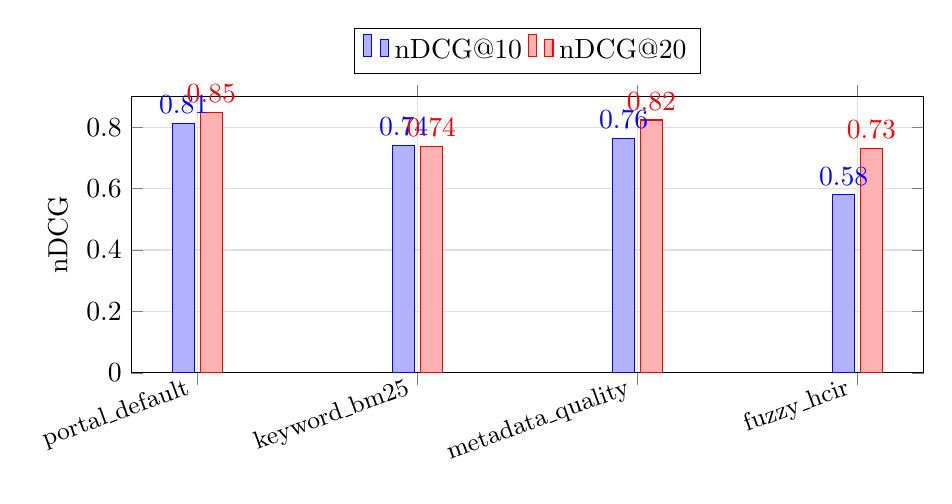
\begin{tikzpicture}
\begin{axis}[
    ybar,
    bar width=8pt,
    width=0.96\textwidth,
    height=0.42\textwidth,
    ymin=0,
    ymax=0.90,
    ylabel={nDCG},
    symbolic x coords={portal\_default,keyword\_bm25,metadata\_quality,fuzzy\_hcir},
    xtick=data,
    xticklabel style={rotate=20,anchor=east,font=\small},
    legend style={at={(0.5,1.08)},anchor=south,legend columns=2},
    nodes near coords,
    nodes near coords align={vertical},
    grid=major,
    major grid style={draw=gray!25}
]
\addplot coordinates {
    (portal\_default,0.8129)
    (keyword\_bm25,0.7393)
    (metadata\_quality,0.7631)
    (fuzzy\_hcir,0.5796)
};
\addplot coordinates {
    (portal\_default,0.8489)
    (keyword\_bm25,0.7370)
    (metadata\_quality,0.8233)
    (fuzzy\_hcir,0.7305)
};
\legend{nDCG@10,nDCG@20}
\end{axis}
\end{tikzpicture}
\caption{nDCG comparison across retrieval systems}
\label{fig:ndcg-bars}
\end{figure}

\section{Deep Analysis}

\subsection{Performance Pattern Analysis}

The aggregate metrics indicate a non-trivial behavior:

\begin{itemize}[leftmargin=1.5em]
  \item \textbf{Best overall in current run:} \texttt{portal_default} is the top system across MAP, P@10, R@10, nDCG@10, nDCG@20, and MRR.
  \item \textbf{Fuzzy vs. keyword baseline:} \texttt{fuzzy_hcir} improves MAP by +4.7\% over \texttt{keyword_bm25} (0.8367 vs 0.7992), but is lower on P@10, R@10, nDCG@10, and MRR.
  \item \textbf{Depth sensitivity:} \texttt{fuzzy_hcir} shows the largest positive rank-depth gain in nDCG (+0.1508 from @10 to @20), suggesting better quality accumulation deeper in the ranking than at the top positions.
  \item \textbf{Interpretation:} The current fuzzy configuration appears to emphasize broader graded relevance coverage at deeper ranks, while top-rank precision remains a tuning target.
\end{itemize}

\subsection{Data and Evaluation Effects}

The judgment distribution is skewed toward grades 2 and 3 (80.0\% combined), and only 1.8\% of labels are grade 0. This can inflate absolute metric values for systems that retrieve many semantically adjacent datasets. As a consequence, comparative claims should prioritize relative differences between systems and include future robustness checks with stricter negative-label sampling.

\subsection{Implications for Phase 4}

The results support two immediate next steps:

\begin{enumerate}[leftmargin=1.5em]
  \item Tune fuzzy membership boundaries and rule weights for top-rank quality (especially @10 metrics).
  \item Replace or complement heuristic judgments with multi-rater human judgments to reduce labeling bias and improve external validity.
\end{enumerate}

\section{User Study Details}

\subsection{Current Status in Repository}

The repository includes user-study related scaffolding:
\begin{itemize}[leftmargin=1.5em]
  \item Annotation tool: \texttt{\detokenize{evaluation/annotation_tool.py}}
  \item Ground truth folder: \texttt{\detokenize{evaluation/ground_truth/}}
  \item Rater folder: \texttt{\detokenize{evaluation/raters/}}
\end{itemize}

At the moment, the \texttt{raters} folder is empty and the available labels in \texttt{ground_truth_auto.json} are heuristic. Therefore, a full human-subject user study has not yet been executed in this workspace snapshot.

\subsection{Planned User Study Protocol}

To complete the thesis evaluation rigorously, the following protocol is specified:

\begin{enumerate}[leftmargin=1.5em]
  \item Recruit 15--20 participants with mixed data-literacy backgrounds.
  \item Use a within-subjects design where each participant evaluates multiple systems.
  \item Present benchmark queries and randomized result lists to reduce order effects.
  \item Collect per-result relevance judgments on a graded scale (0--3).
  \item Collect trust and usability perceptions after each system condition.
  \item Compute inter-rater reliability (e.g., Cohen's/Fleiss' kappa).
  \item Recompute IR metrics using human labels and compare with heuristic-label outcomes.
\end{enumerate}

\subsection{Proposed Study Outputs}

The user study should produce:
\begin{itemize}[leftmargin=1.5em]
  \item Cleaned rater-level judgments per query/result.
  \item Agreement statistics and conflict analysis.
  \item Human-labeled benchmark release for reproducibility.
  \item Updated comparative tables and significance testing.
\end{itemize}

\section{Validation Status}

The current implementation has been validated at two levels:

\begin{itemize}[leftmargin=1.5em]
  \item \textbf{Static validation:} The codebase reports no errors in the checked Python files.
  \item \textbf{Integration validation:} The end-to-end integration test passed with all expected checkpoints.
  \item \textbf{Evaluation artifact validation:} Metric files, benchmark query set, and auto-labeled ground truth are present and internally consistent (15 queries, 450 judgments).
\end{itemize}

The integration test confirms that the fuzzy engine, query parser, ranking layer, baseline systems, explanation generator, and configuration layer are all functioning in the current workspace state.

\section{Known Gaps and Boundaries}

The prototype is operational, but the documentation should remain precise about what has and has not been fully completed:

\begin{itemize}[leftmargin=1.5em]
  \item The implemented prototype is available and runnable through Streamlit.
  \item Evaluation artifacts exist in the repository, but a full Phase 3 user study is not yet documented in the current workspace.
  \item The semantic baseline includes a stubbed or fallback implementation in places, so future work may still refine the AI comparison path.
\end{itemize}

\section{Conclusion}

Phase 3 has successfully produced a working prototype for the Swiss OGD fuzzy retrieval system. The system now supports query parsing, metadata retrieval, fuzzy ranking, baseline comparison, and explanation generation. The verified integration results show that the prototype stack is internally consistent and ready for the evaluation-focused work that follows in the thesis process.

\section{References}

\begin{thebibliography}{9}

\bibitem{zadeh1965}
L. A. Zadeh, ``Fuzzy sets,'' \emph{Information and Control}, vol. 8, no. 3, pp. 338--353, 1965.

\bibitem{mamdani1974}
E. H. Mamdani, ``Application of fuzzy algorithms for control of simple dynamic plant,'' \emph{Proceedings of the Institution of Electrical Engineers}, vol. 121, no. 12, pp. 1585--1588, 1974.

\bibitem{hevner2004}
A. R. Hevner, S. T. March, J. Park, and S. Ram, ``Design science in information systems research,'' \emph{MIS Quarterly}, vol. 28, no. 1, pp. 75--105, 2004.

\bibitem{peffers2007}
K. Peffers, T. Tuunanen, M. A. Rothenberger, and S. Chatterjee, ``A design science research methodology for information systems research,'' \emph{Journal of Management Information Systems}, vol. 24, no. 3, pp. 45--77, 2007.

\bibitem{manning2008}
C. D. Manning, P. Raghavan, and H. Sch{"u}tze, \emph{Introduction to Information Retrieval}. Cambridge University Press, 2008.

\bibitem{opendataswiss}
opendata.swiss, ``Swiss Open Government Data Portal,'' \url{https://opendata.swiss/}.

\end{thebibliography}

\end{document}